\documentclass[letterpaper]{article}
\usepackage[czech]{babel}
\usepackage[utf8]{inputenc}
\usepackage[unicode]{hyperref} % na začátku bylo místo unicode bookmark
\usepackage[chorded]{songs}
\usepackage{geometry}
\usepackage{float}



% Pokud je \rf[čislo], tak se opakuje číslokrát, jinak jednou.
\newcommand\rf[1][\relax]{\ifx\relax#1 
	\beginverse* \textbf{Ref.}\\ \endverse 
	\else 
		\beginverse* \textbf{Ref.} \rep{#1}\\ \endverse 
\fi}


% \includeonlysongs{2}
\setlength\baselineadj{-\baselineskip}
\setlength{\oddsidemargin}{0in}
\setlength{\evensidemargin}{0in}
\setlength{\textwidth}{6.5in}
\setlength{\topmargin}{0in}
\setlength{\topskip}{0in}
\setlength{\headheight}{0in}
\setlength{\headsep}{0in}
\setlength{\textheight}{9.1in}
\settowidth{\versenumwidth}{1.\ }
%\pagestyle{empty}

\newindex{titleidx}{cbtitle}
\newindex{entitleidx}{encbtitle}
\indexsongsas{titleidx}{\thepage}
\indexsongsas{entitleidx}{\thepage}

\nosongnumbers
%\songcolumns{3}

% START HEADER SECTION
\usepackage{fancyhdr}
\pagestyle{fancy}
\chead{}
\rhead{}
%\fancyhf{}
\renewcommand{\headrulewidth}{0pt} % removes header line
\lhead{\hyperlink{page.2}{$\leftarrow$}}
% END HEADER SECTION

\usepackage{graphicx}
\begin{document}
\thispagestyle{empty}
Místo pro úvodní stránku.
%\begin{figure}[H]
%	\centering
%	\scalebox{0.7}{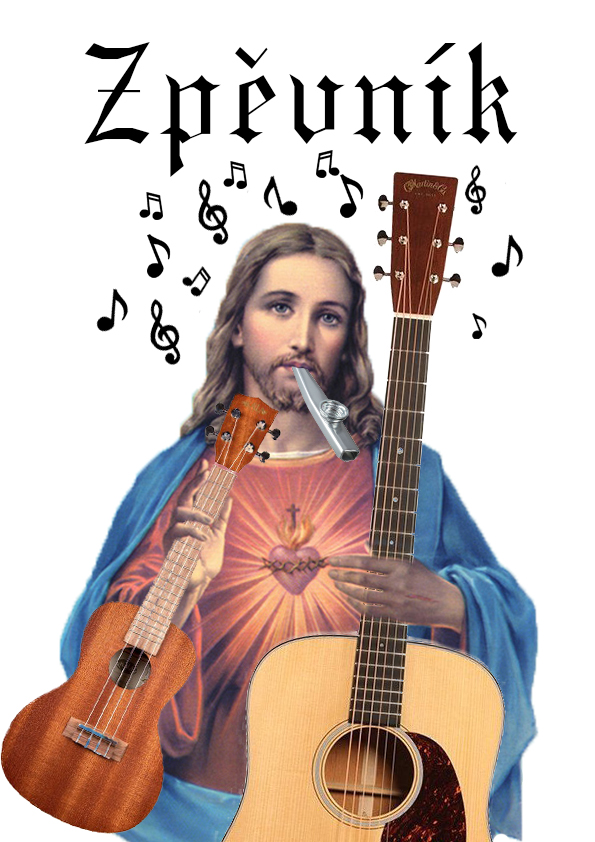
\includegraphics{title_picture.jpg}}

	%\scalebox{0.7}{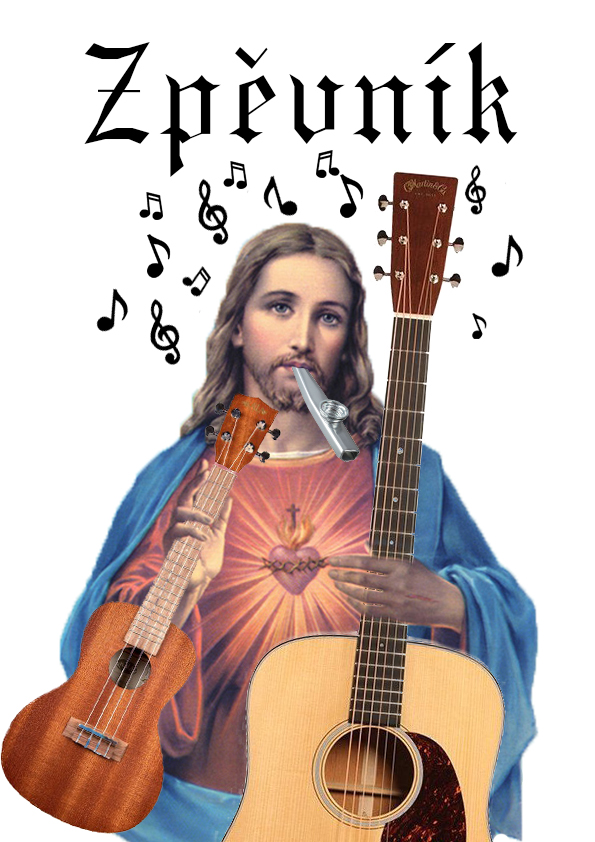
\includegraphics{title_picture.jpg}}
%\end{figure}
\vspace*{\fill}
Vygenerováno: \today

\newpage

\thispagestyle{empty} % removes refference
\showindex[3]{Obsah}{titleidx}
\thispagestyle{empty}
\showindex[3]{Cizojazyčné - obsah}{entitleidx}

\songsection{České písničky}
\begin{songs}{titleidx}
\input{songs/merged_cze_songs.sbd}
\end{songs}

\songsection{Anglické písničky}
\begin{songs}{entitleidx}
	\input{songs/merged_eng_songs.sbd}
\end{songs}

\end{document}

